\chapter{Results}

\begin{center}
    \textit{This chapter presents the outcomes of the project, including the functionality and performance of the developed application. It highlights the achieved results in relation to the project goals and requirements.}
\end{center}

\section{Overview of Delivered Product}
The delivered product refers to the final version of the application submitted at the conclusion of this Bachelor’s thesis. The application was developed at the request of the product owner and based on the requirements provided. The initial description served as a general concept rather than a detailed specification, which meant that decisions regarding design, architecture, and technology were left to the development team. Throughout the development process, ideas and design choices were discussed with the product owner and approved during regular meetings. \\

The application was developed as an open-source project with the intention that the code can be reused, maintained, and extended by others. All components are built using open and freely available technologies, ensuring that the system can be installed on local hardware without the need for licensed software or cloud-based services. This aligns with the requirement that all processing should be performed locally, using common hardware such as a webcam connected to a local machine running either Windows or Ubuntu. \\

The project follows clear coding standards and development best practices, making the code easy to understand and modify. All functionality is well documented, enabling future developers to build upon the existing solution. For example, to support new chess variants, integrate additional hardware, or improve the recognition models. To support future development and accessibility, the source code is published in a public Git repository without restrictions on reuse or adaptation. \\

The application itself is a local, camera-based system for digitalizing over-the-board chess games in real time. It detects piece movements on a physical chessboard using image recognition and converts the game into a PGN file, which can be viewed or analyzed digitally. The system operates entirely on local hardware, with a front-end interface that allows users to follow games live and a back-end that manages board recognition and game logic. The application is designed to be low-cost, open-source, and easy to maintain, with extensibility in mind for future features.

\section{Functional Results}
The application consists of three main components: machine learning, WebSocket communication, and the front-end interface. The back-end handles image recognition and game logic, using a machine learning model to detect board states. It communicates with the front-end through a WebSocket connection. The front-end is responsible for presenting this information to the user in real time. The cameras is connected with a USB-hub, where multiple cameras can be attached to the same computer. 

\subsection{Machine Learning}
To be completed.

\subsection{API}
To enable real-time updates and improve the responsiveness of the front-end interface, the application uses a WebSocket connection between the back-end and the front-end. This method was suggested by the product owner and was also approved by the supervisor. This communication channel is used for transmitting move data as it is detected by the board recognition system. Unlike traditional HTTP requests, which operate on a request-response basis, WebSocket allows for continuous, two-way communication between the server and the client. \\

Once the application initiates a connection, the WebSocket remains open throughout the session. As new moves are identified on the physical board, the back-end sends the corresponding move data as messages through the WebSocket. These messages are then received by the front-end, which updates the displayed move list and board state in real time. This provides a seamless viewing experience for users following live games. \\

The WebSocket server also handles specific command messages. For example, when the server sends a message labeled "RESET," the front-end clears the current move list, typically indicating the start of a new game. A message labeled "INVALID" is used to signal an unrecognized or incorrect move and does not trigger any front-end changes. All other messages are assumed to be valid algebraic notation representing chess moves and are appended to the game history displayed to the user. \\

The WebSocket functionality is encapsulated in a custom React hook on the front-end, which manages the connection lifecycle and state updates. This abstraction simplifies integration into the user interface and ensures that resources are properly cleaned up when the component is unmounted. Overall, the use of WebSocket communication is a key component in delivering a responsive and live experience, particularly for tournaments and public displays where move-by-move tracking is essential.

\subsection{Frontend}
The front-end of the application serves as the user interface. It includes a control panel for tournament organizers and a web application for spectators. The application's main responsibility is to visualize the chessboard and display ongoing moves. The front-end communicates with the back-end via WebSocket to ensure real-time updates and interactivity. \\

The \textbf{control panel} is an administrative tool accessible only to the tournament organizers. It functions as a standalone dashboard application and is available exclusively on the computer that starts the application, as shown in Figure~\ref{fig:control-panel}. This setup ensures that spectators visiting the website cannot access the control panel. \\

\begin{figure}[h!] \centering 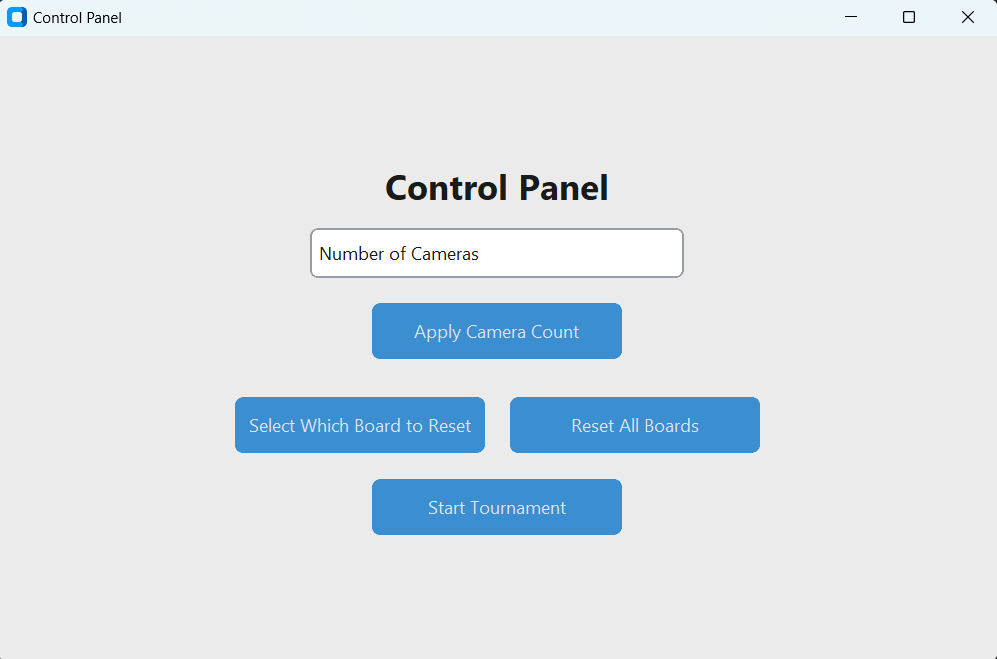
\includegraphics[width=0.75\linewidth]{figures/results/frontend/control-panel/control-panel.png} \caption[Control panel for tournament organizers]{The control panel used by the tournament organizers.}\label{fig:control-panel} \end{figure}

Before the tournament begins, the organizer must start the application and configure it using the control panel. This includes specifying the number of cameras to be used, allowing the application to connect to the appropriate number of video feeds. When the number of selected cameras is connecting, a progress bar is visible for the user, as shown in Figure~\ref{fig:control-panel-camera} Once the connections are established, the tournament can be started by pressing the "Start Tournament" button. \\
 
\begin{figure}[h!] \centering 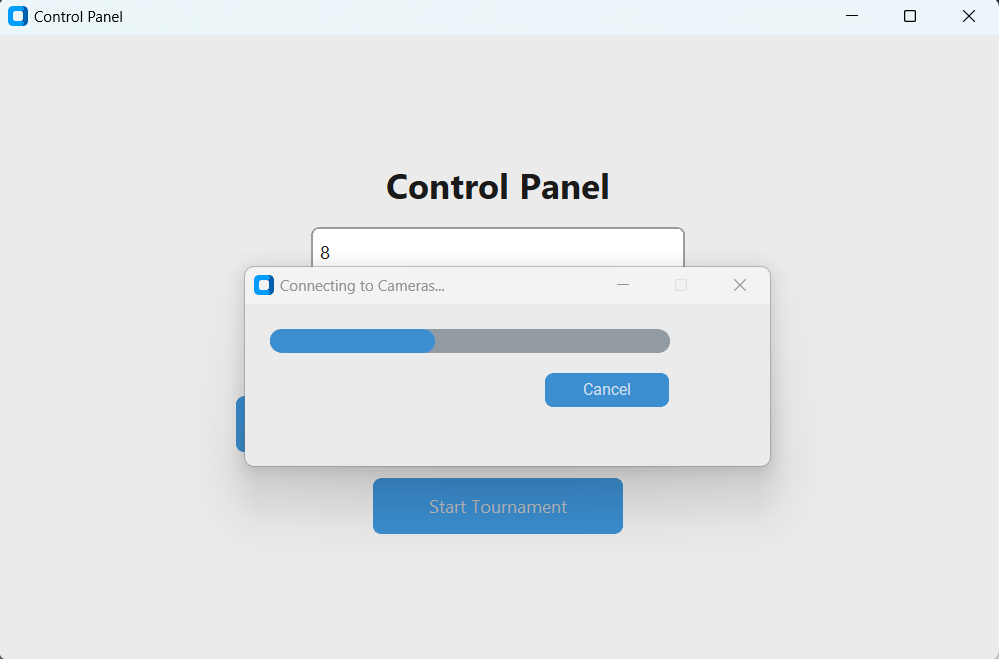
\includegraphics[width=0.75\linewidth]{figures/results/frontend/control-panel/camera-progress.png} \caption[Progress bar for camera connections]{A progress bar representing the status of connecting cameras}\label{fig:control-panel-camera} \end{figure}

When completed connecting the cameras successfully, a success message is displayed, as shown in Figure~\ref{fig:control-panel-camera-success}. If the organizer attempts to connect more cameras than the system can detect, an error message is displayed, as shown in Figure~\ref{fig:control-panel-camera-error}. This provides feedback to the user about what went wrong. For example, the message "Error: Could not open Camera 1" indicates that the system could not find a camera with ID 1. In the illustrated scenario, no cameras were connected, which caused the error to appear. \\

\begin{figure}[h!] \centering 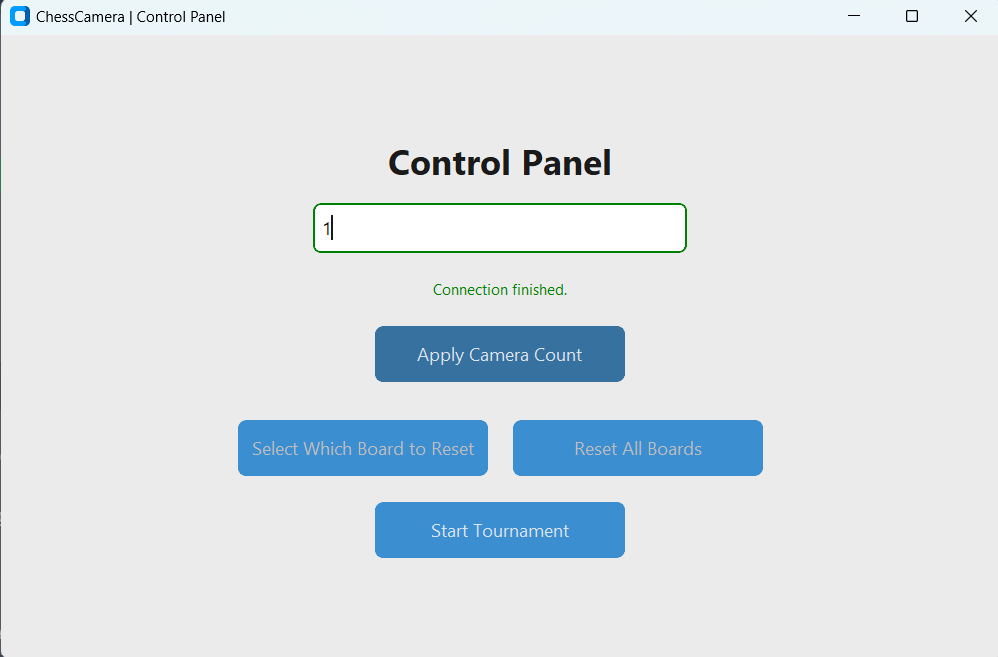
\includegraphics[width=0.75\linewidth]{figures/results/frontend/control-panel/camera-success.png} \caption[Success message for camera connections]{A success message for  connecting cameras correctly}\label{fig:control-panel-camera-success} \end{figure}

\begin{figure}[h!] \centering 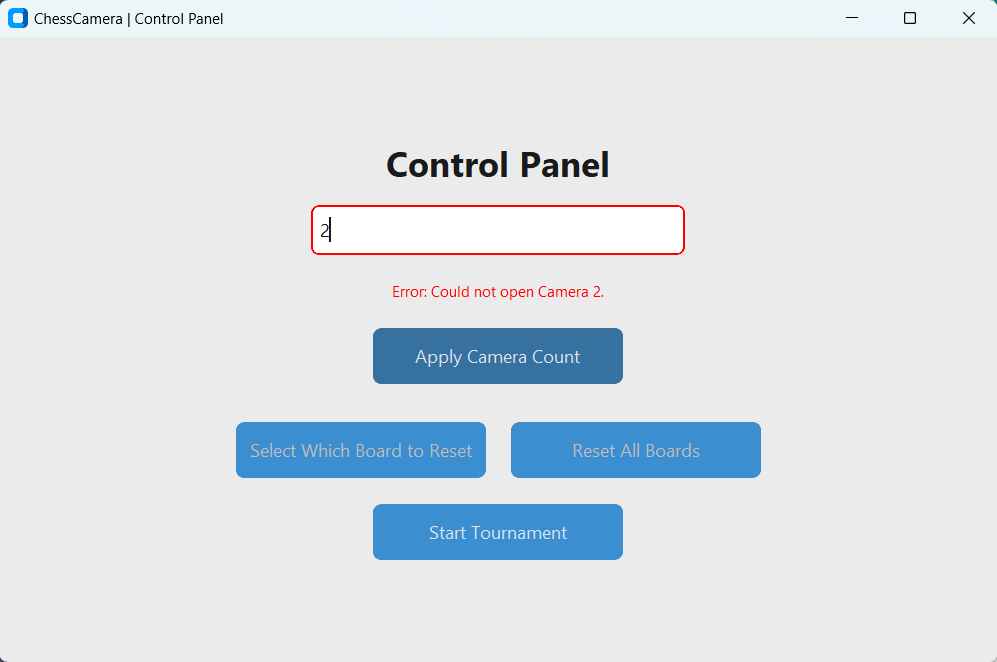
\includegraphics[width=0.75\linewidth]{figures/results/frontend/control-panel/camera-error.png} \caption[Error message for camera connections]{A error message for failure connecting cameras}\label{fig:control-panel-camera-error} \end{figure}

The control panel also provides functionality for resetting individual boards or all boards simultaneously. When a tournament round is finished, the organizers must reset all boards before the next round can begin. By pressing the "Reset All Boards" button, they can reset all connected boards at once. In some scenarios, it may be necessary to reset a single board. In such cases, the organizers can use the "Select Which Board to Reset" feature, as shown in Figure~\ref{fig:control-panel-reset-boards}. \\

\begin{figure}[h!] \centering 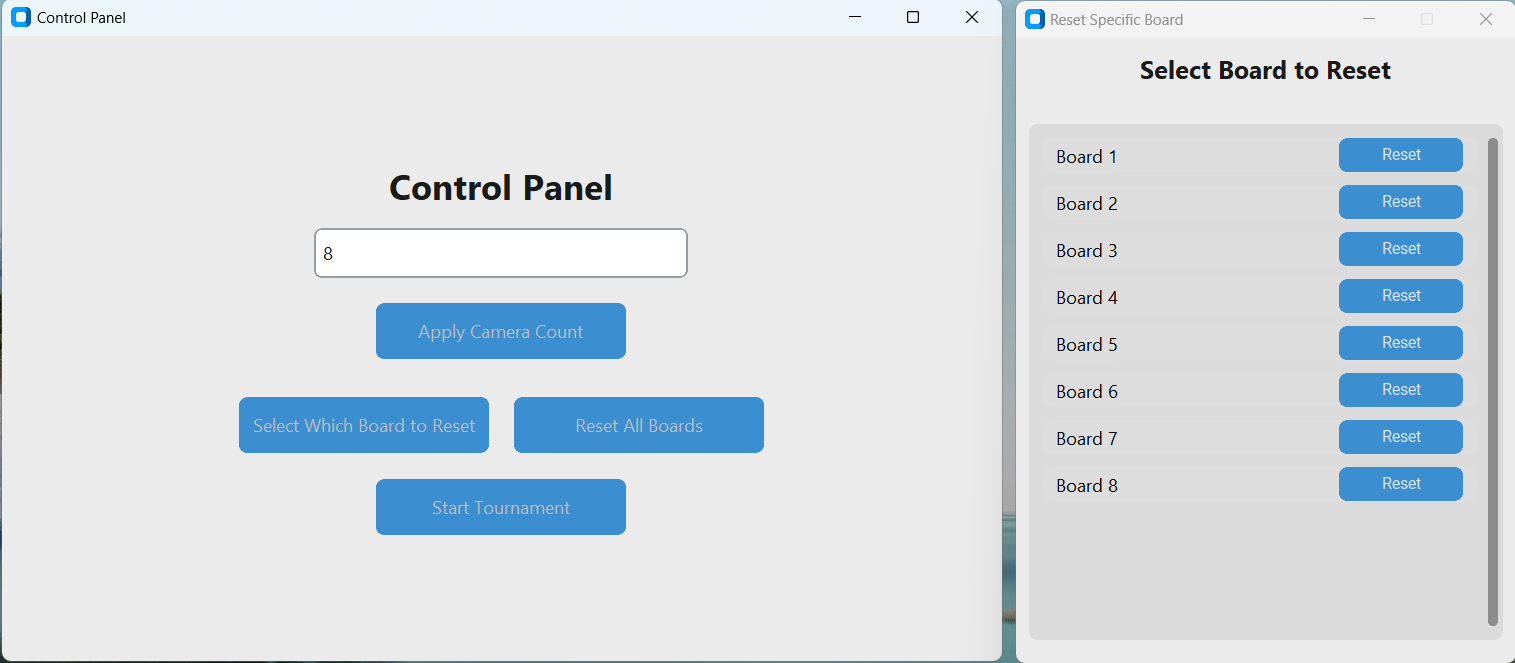
\includegraphics[width=0.75\linewidth]{figures/results/frontend/control-panel/reset-boards.png} \caption[Panel to reset a single board]{The panel to select which board to be reset}\label{fig:control-panel-reset-boards} \end{figure}

The \textbf{web application} was designed for spectators  who want to follow the tournament and watch the games being played. It includes several features that present the tournament in a user-friendly manner. These include a Tournament View, which displays a table of all ongoing games; a Game Preview page with summaries of each game; and a Board View, which shows the chessboard, \gls{pgn} display, and a live camera feed for a specific board. The application also contains a header with links to informational pages such as "How it Works", which explains how to use the system, and "About", which outlines the project’s purpose and requirements. \\

The application is implemented as a \textbf{responsive} web application that functions on both desktop and mobile devices. The layout adapts to different screen sizes, which helps maintain usability across platforms. Key interface elements such as navigation, buttons, and forms adjust to fit smaller screens, making it possible to use the application on smartphones and tablets as well. It also includes an option to switch between light and dark color modes. This setting can be changed in the system preferences and allows users to choose the visual style they find more comfortable. The color palettes are adjusted accordingly, providing a consistent appearance throughout the interface depending on the selected mode. \\

For demonstration purposes, a \textbf{dataset} of chess players was created and displayed in the Tournament View. This dataset includes real professional chess players along with their corresponding ratings, in order to simulate multiple boards and games. Since the available hardware for testing was limited to only two cameras, a mocked dataset was used to represent additional boards and players during the demonstration. \\

When the application is started, both the control panel and the web application launch simultaneously. This means the web application is accessible even before the tournament has officially started. Upon entering the web application, the initial page shown is the \textbf{Tournament View}. If the tournament has not yet started, this view contains no data. To provide visual feedback to spectators while they wait, a loading animation is displayed, as shown in Figure~\ref{fig:tournament-view-loading}.\\

\begin{figure}[h!] \centering \fbox{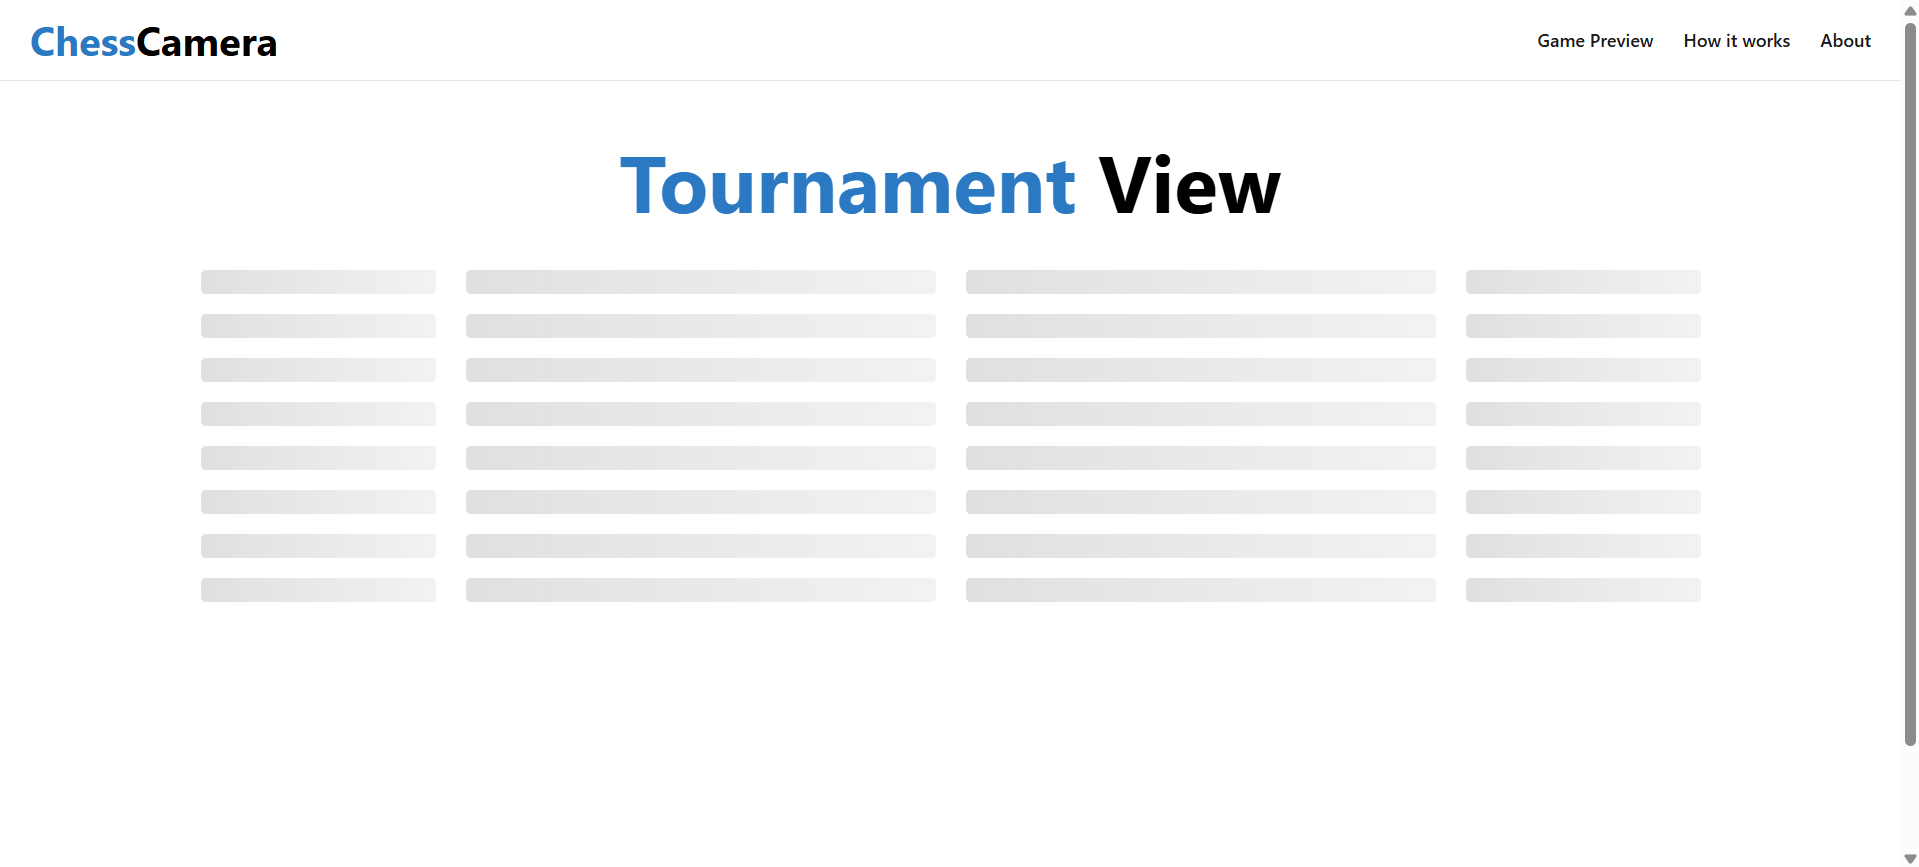
\includegraphics[width=0.75\linewidth]{figures/results/frontend/tournament-view/loading.png}}\caption[Loading animation]{A loading animation shown while waiting for the tournament to begin.}\label{fig:tournament-view-loading} \end{figure}

When the tournament is started, the list of available boards is displayed in place of the loading screen, as shown in Figure~\ref{fig:tournament-view-mocked}. This Tournament View serves as an overview of all active games in the tournament. Each row in the table represents a board, showing the board number, the name of the white and black players, and their respective ratings. The layout is designed to be clean and readable, with alternating row colors for better visual distinction. Player names and ratings are displayed prominently to give spectators an immediate sense of who is playing. At the far right of each row is a "LIVE" button. When clicked, this button redirects the user to the corresponding Board View, where they can watch the specific game in real time. \\

\begin{figure}[h!] \centering \fbox{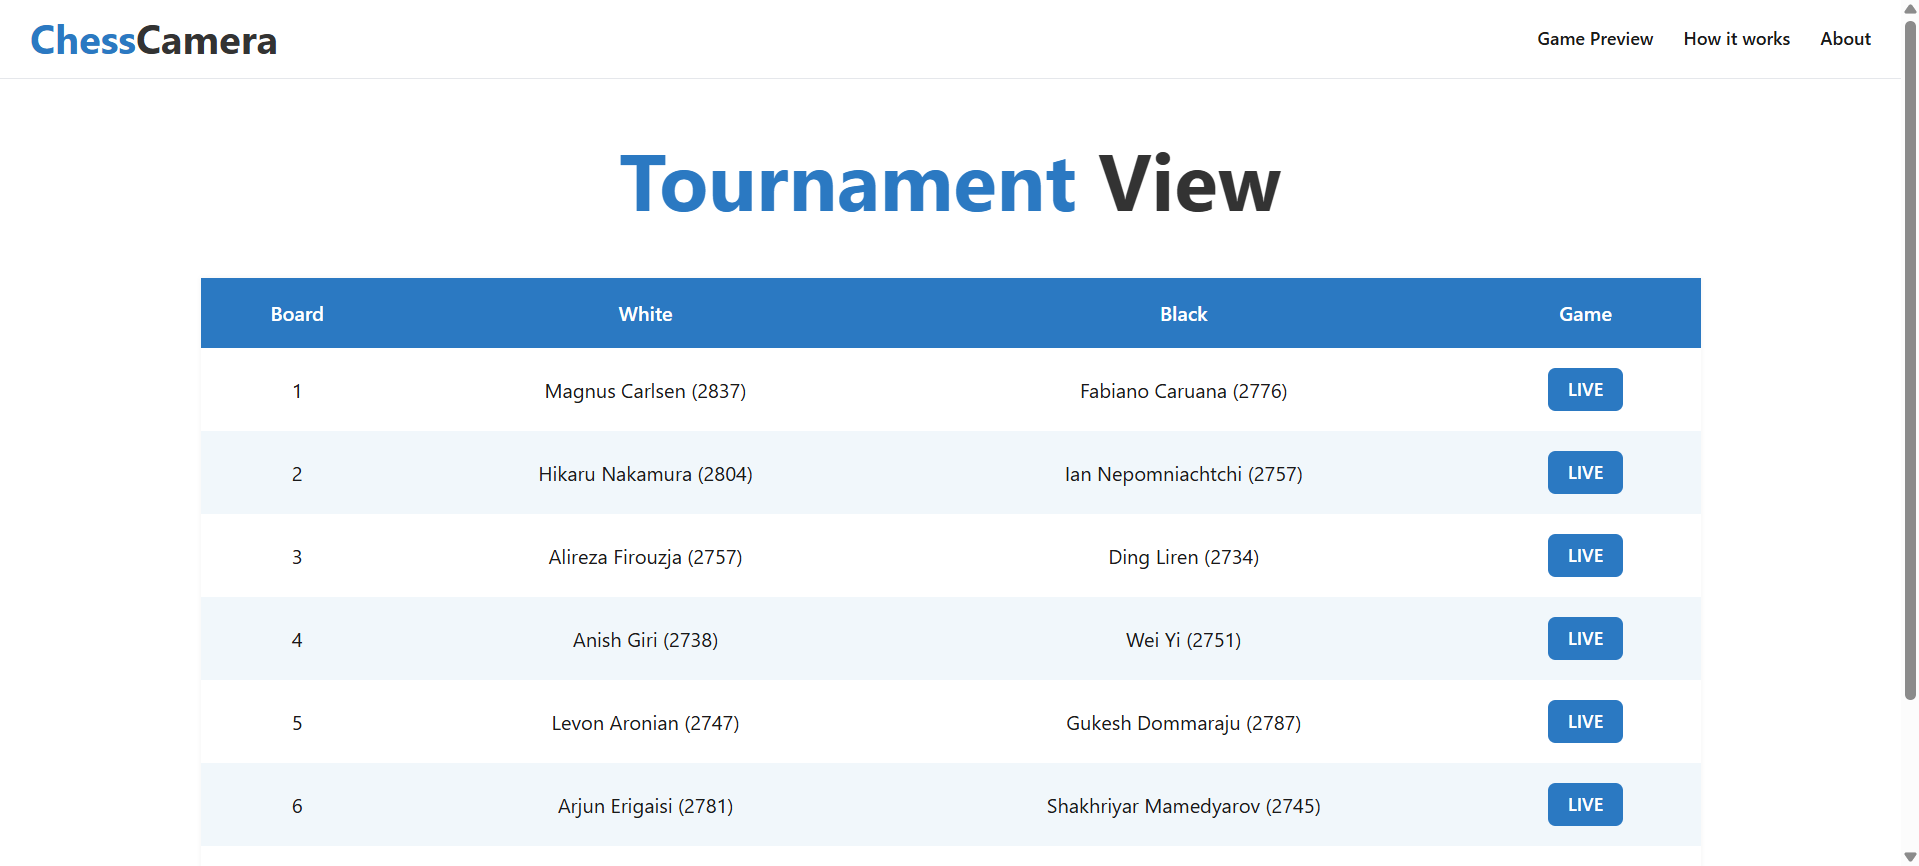
\includegraphics[width=0.75\linewidth]{figures/results/frontend/tournament-view/mocked.png}}\caption[Display of tournament]{A mocked demonstration of a tournament display.}\label{fig:tournament-view-mocked} \end{figure}

The Tournament View automatically adjusts its layout when displayed on smaller screens, such as smartphones or tablets. In this mobile view, the table format used in the desktop version is replaced by a more compact, vertically stacked layout. This design makes the content easier to read and interact with on narrow screens. The loading screen remains visually similar but is scaled to fit the smaller display, as shown in Figure~\ref{fig:small-tournament-view-loading}. When the tournament begins, each game is presented as a vertical card, where key details, such as board number, player names, and the “LIVE” button, are reorganized to fit within the available width, as shown in Figure~\ref{fig:small-tournament-view}. This layout enhances readability and usability on mobile devices without reducing the overall functionality of the view. \\

\begin{figure}[h!]
    \centering
    \begin{subfigure}[h!]{0.4\linewidth}
        \centering
        \fbox{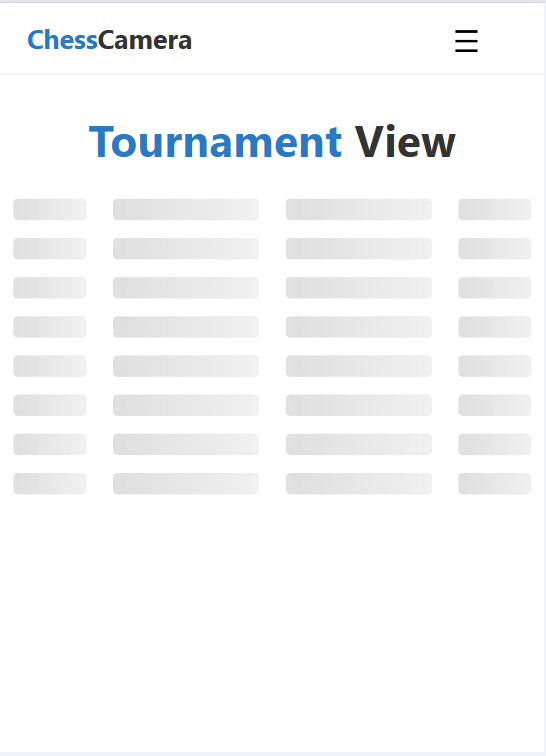
\includegraphics[width=\linewidth]{figures/results/frontend/tournament-view/loading-mobile.png}}
        \caption{Loading screen}
        \label{fig:small-tournament-view-loading}
    \end{subfigure}
    \hfill
    \begin{subfigure}[h!]{0.4\linewidth}
        \centering
        \fbox{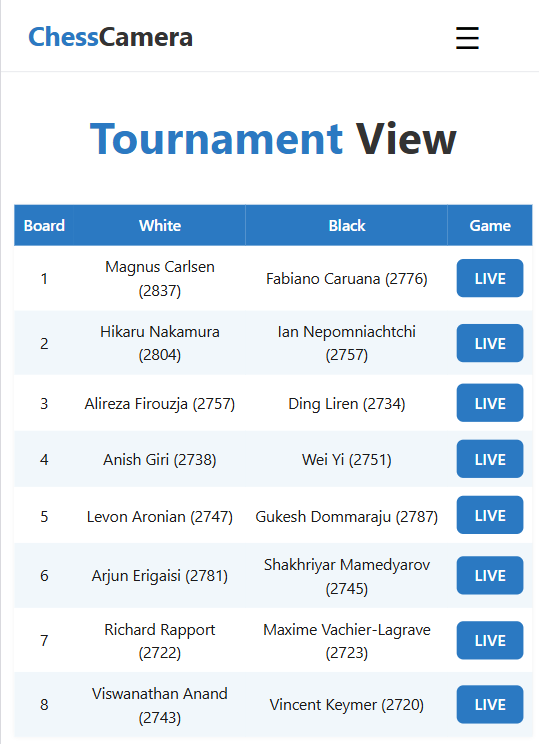
\includegraphics[width=\linewidth]{figures/results/frontend/tournament-view/mocked-mobile.png}}
        \caption{Mocked data}
        \label{fig:small-tournament-view}
    \end{subfigure}
    \caption{Tournament View on smaller screen}
    \label{fig:small-view-tournament-view-group}
\end{figure}

The \textbf{Board View} presents a detailed interface for following a specific game. It combines multiple visual elements to enhance the spectator experience, as shown in Figure~\ref{fig:board-view-mocked}. On the left side, a live camera feed shows the physical chessboard and players, offering a real-world perspective of the game. Alongside this is a \gls{pgn} display that lists all moves played so far. In the center, a digital chessboard displays the current state of the game, updated in real time as moves are made. To the right, an evaluation bar provides a visual indication of which player is currently favored based on the position, helping users understand the balance of the game without advanced chess knowledge. \\

\begin{figure}[h!] \centering \fbox{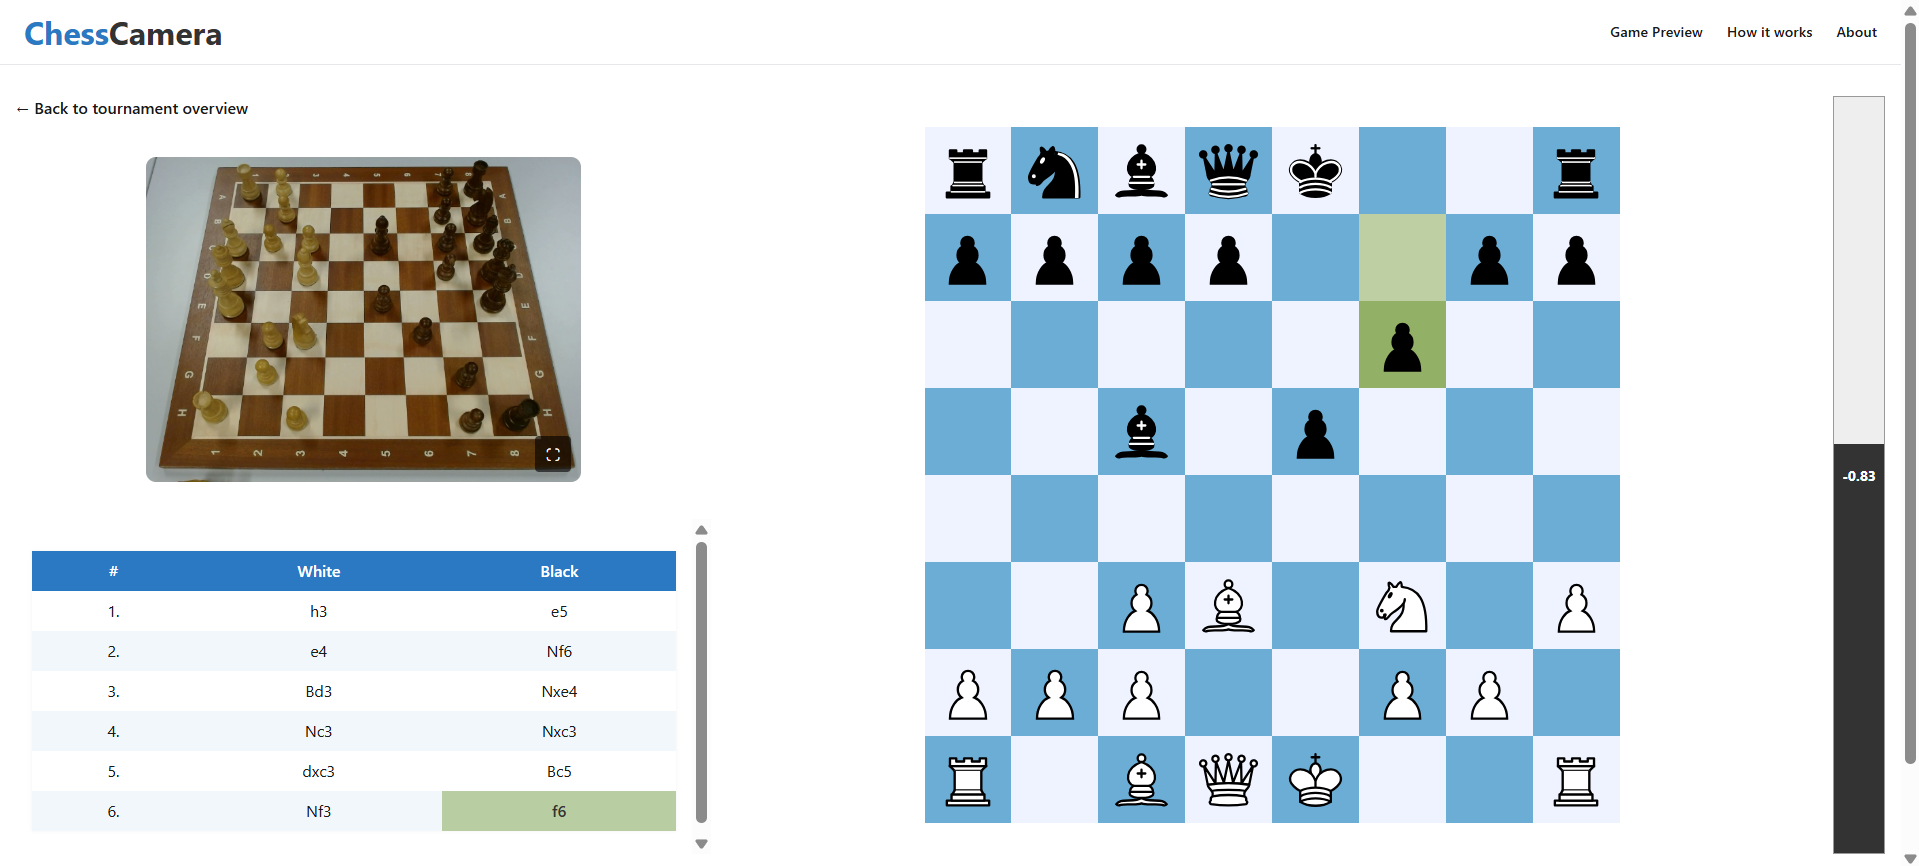
\includegraphics[width=0.75\linewidth]{figures/results/frontend/board-view/desktop.png}}\caption[Display of a board]{A mocked demonstration of an active game}\label{fig:board-view-mocked} \end{figure}

Each board in the tournament has its own unique URL, following the format http://localhost:5173/board/{id}, where {id} corresponds to the board number. This allows spectators to directly access a specific game's Board View by navigating to its dedicated link, enabling easy sharing of individual games. \\

The Board View includes several interactive and dynamic elements that enhance the spectator experience beyond static game updates. The live camera feed is displayed in the left section of the interface and can be expanded to a larger view if desired. This allows spectators to get a closer look at the physical chessboard and players, offering a more immersive viewing experience, as shown in Figure~\ref{fig:camera-fullscreen}. \\

\begin{figure}[h!] \centering \fbox{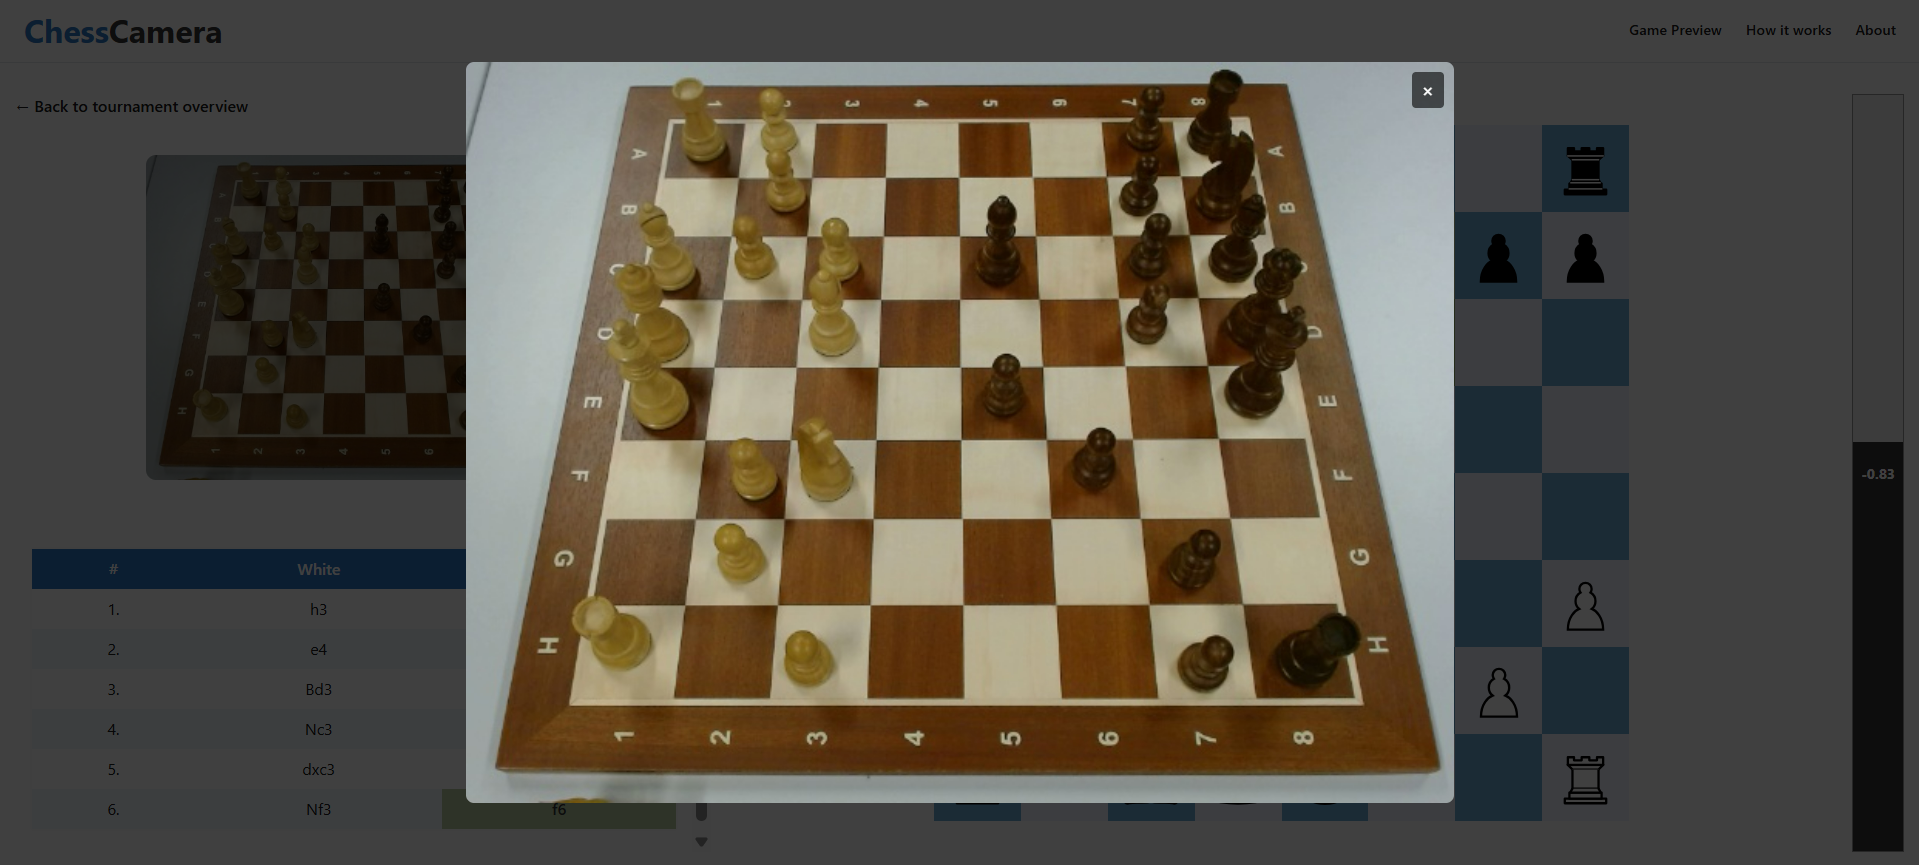
\includegraphics[width=0.75\linewidth]{figures/results/frontend/board-view/camera-fullscreen.png}}\caption[Camera in full screen]{Expanded camera in full screen}\label{fig:camera-fullscreen} \end{figure}

As the game progresses, the \gls{pgn} display updates in real time. It lists all moves made so far in a table, where the most recent move is visually marked. This is to help users follow the flow of the game without needing to track moves manually. The digital chessboard is also updated live. When a move is made, the board highlights both the square the piece moved from and the square it moved to, visually representing the last action taken. This helps spectators quickly identify changes in the game state. To the right of the board, an evaluation bar gives a quick visual indication of which player currently has the best position. This feature uses a vertical bar to indicate which player has the advantage. A higher bar toward the top or bottom signals a better position for White or Black, respectively. This makes it easier for casual viewers to understand the competitiveness of the game without requiring deep chess knowledge. \\

Like the Tournament View, the Board View also adapts to smaller screens through a responsive layout. However, the adjustments in this view are more noticeable due to the limited space and size of the elements. The layout is prioritized based on typical spectator preferences, where the digital chessboard remains the central focus. Since the main purpose of this view is to present the ongoing game on a digital board, it is positioned at the top for maximum visibility on smaller screens. \\

Below the chessboard is the \gls{pgn} display, which shows the list of moves played. In contrast to the desktop layout, where the moves may be presented in a table format, the layout for smaller screens uses a vertical list to create a cleaner and more compact presentation. This makes the move history easier to read on narrow screens, while still maintaining clarity, as shown in Figure~\ref{fig:small-board-view}. \\

At the bottom of the screen is the camera feed. While it is not as highly prioritized as the board or move list, it remains available to users who want a live view of the game. The live camera can also be expanded to full screen for a closer look, as demonstrated in Figure~\ref{fig:small-board-view-camera-expanded}. This layout ensures that all core features remain accessible, while optimizing the viewing experience for mobile users. \\

\begin{figure}[h!]
    \centering
    \begin{subfigure}[h!]{0.4\linewidth}
        \centering
        \fbox{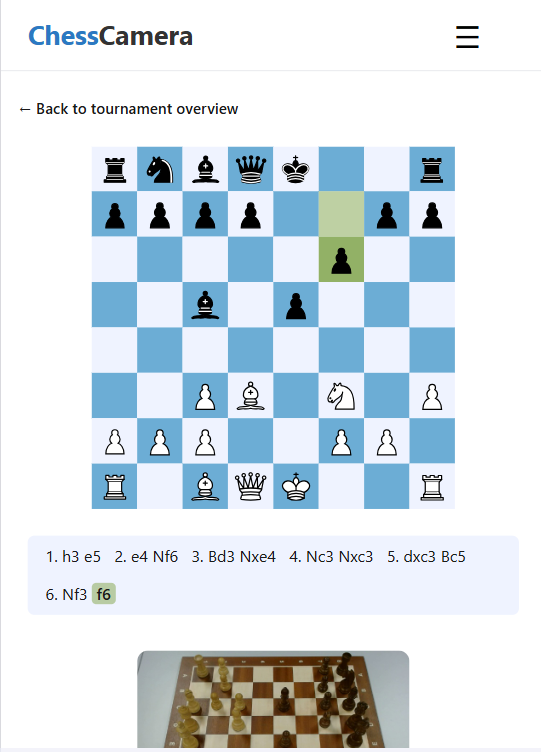
\includegraphics[width=\linewidth]{figures/results/frontend/board-view/mobile.png}}
        \caption{Mocked data}
        \label{fig:small-board-view}
    \end{subfigure}
    \hfill
    \begin{subfigure}[h!]{0.4\linewidth}
        \centering
        \fbox{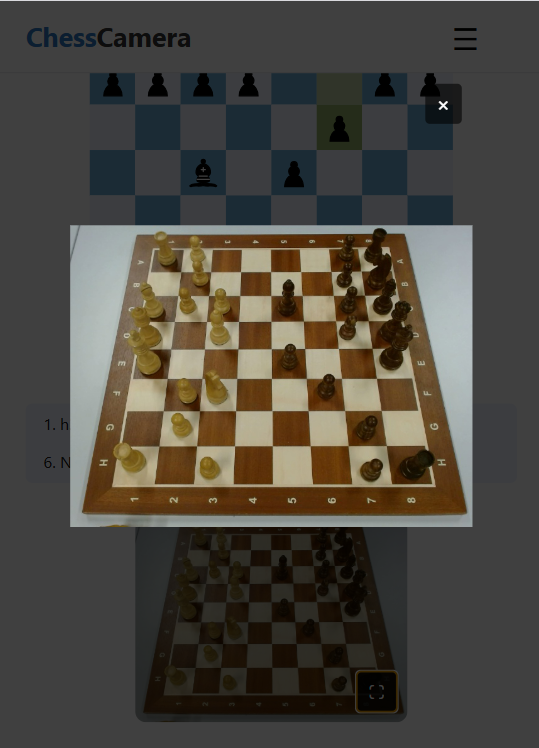
\includegraphics[width=\linewidth]{figures/results/frontend/board-view/camera-fullscreen-mobile.png}}
        \caption{Camera expanded when in smaller screen}
        \label{fig:small-board-view-camera-expanded}
    \end{subfigure}
    \caption{Board View on smaller screen}
    \label{fig:small-view-board-view-group}
\end{figure}

The application includes a \textbf{navigation header} that remains consistent across all pages. This header provides quick access to key sections of the site, including the Game Preview, How It Works, and About Us pages. On smaller screens, the navigation automatically collapses into a hamburger menu, maintaining a clean and user-friendly interface without reducing accessibility, as shown in Figure~\ref{fig:navigation-header}. \\

\begin{figure}[h!]
    \centering
    \begin{subfigure}[h!]{0.4\linewidth}
        \centering
        \fbox{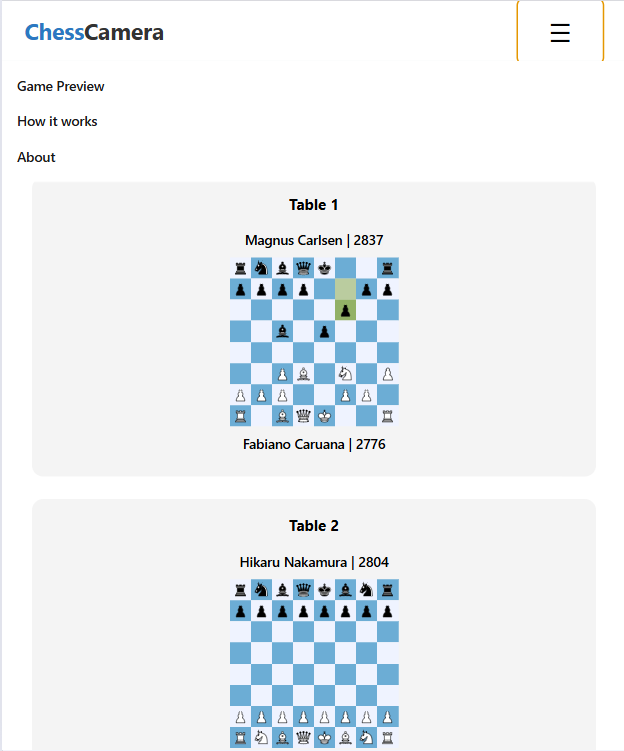
\includegraphics[width=\linewidth]{figures/results/frontend/game-preview/navigation.png}}
        \caption{Navigation header as a hamburger menu on a smaller screen}
        \label{fig:navigation-header}
    \end{subfigure}
    \hfill
    \begin{subfigure}[h!]{0.4\linewidth}
        \centering
        \fbox{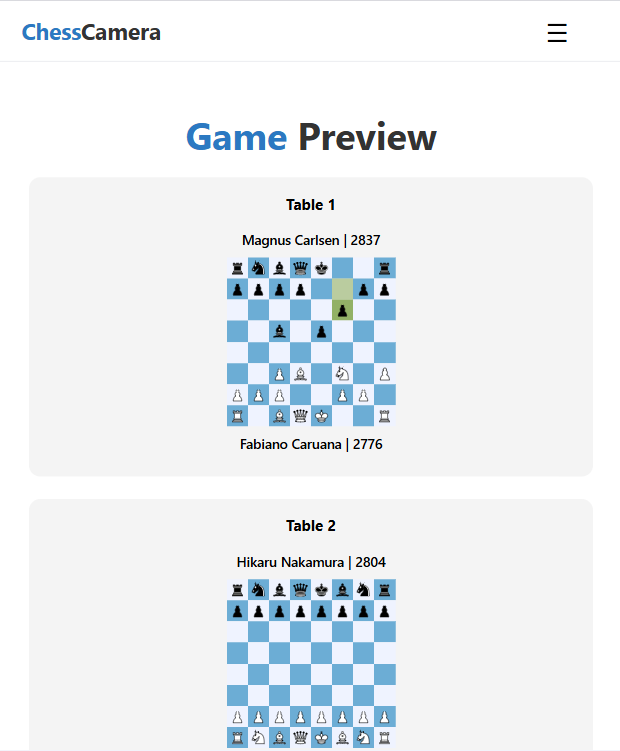
\includegraphics[width=\linewidth]{figures/results/frontend/game-preview/mobile.png}}
        \caption{Game preview on a smaller screen}
        \label{fig:small-game-preview}
    \end{subfigure}
    \caption{Board View on smaller screen}
    \label{fig:small-view-game-preview-group}
\end{figure}

Through the header, spectators can navigate to the \textbf{Game Preview} page. This view shares similarities with the Tournament View but is more focused on highlighting individual games. Instead of displaying all games in a table format, it includes a preview of the currently active game, giving users a quick overview without needing to enter the full Board View, as shown in Figure~\ref{fig:game-preview}.

\begin{figure}[h!] \centering \fbox{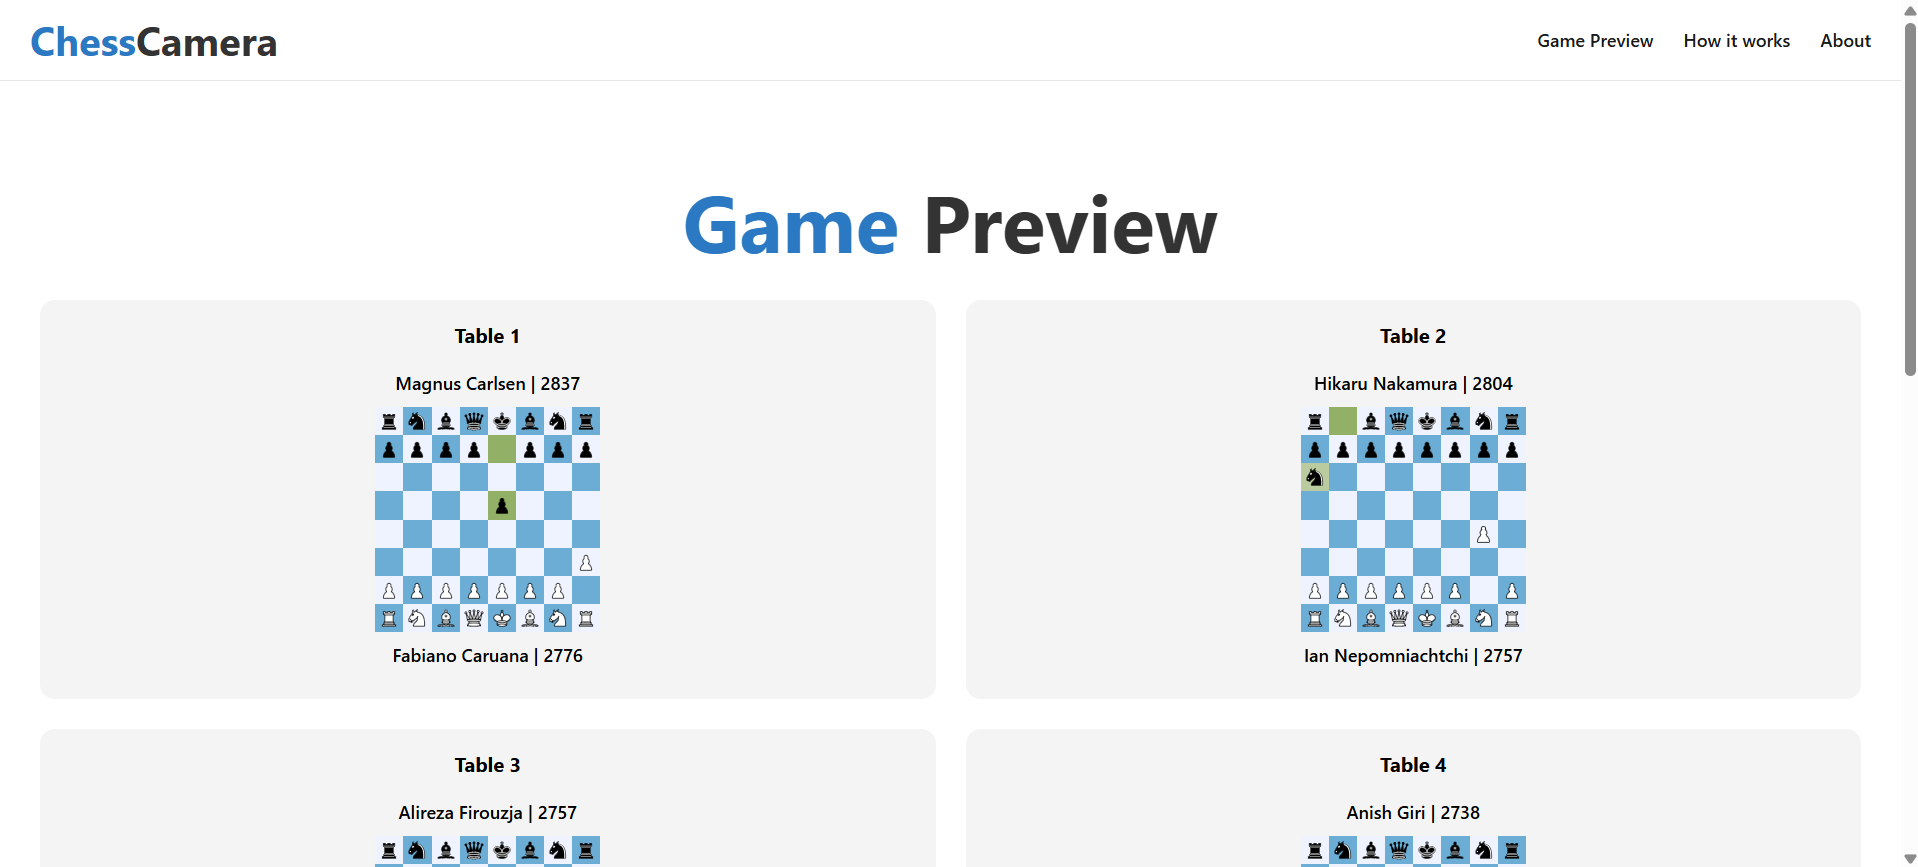
\includegraphics[width=0.75\linewidth]{figures/results/frontend/game-preview/desktop.png}}\caption[Preview of active games]{A mocked demonstration of a game preview page.}\label{fig:game-preview} \end{figure}

\section{Technical Achievements}
Architecture overview (e.g., system diagram, deployment pipeline). Performance metrics (e.g., response time, uptime). Details on scalability, security, or CI/CD if relevant. 

\section{Testing and Quality Assurance}
Summary of testing performed (unit tests, integration tests, manual testing). Test coverage results or bugs discovered/fixed. If relevant, include tables or graphs showing test results or reliability.